\section*{Appendix A - Listings}

\begin{lstlisting}[language=C, caption={Almost Equal algorithm}, label={lst:almost_equal}]
bool almost_equal(float x, float y) {
    int maxUlps = 2048;
    int xBits = *(int *)&x;  // Evil bit level hacking from Quake III Q_sqrt
    int yBits = *(int *)&y;  // Evil bit level hacking from Quake III Q_sqrt
    int minValue = 1 << 31;
    if (xBits < 0) xBits = minValue - xBits;
    if (yBits < 0) yBits = minValue - yBits;

    int difference = xBits - yBits;
    return difference != minValue && fabsf(difference) <= maxUlps;
}
\end{lstlisting}

\begin{lstlisting}[language=C, caption={CPU addition algorithm}, label={lst:cpu_addition}]
bool matrix_addition(matrix_t *matrix_a, matrix_t *matrix_b, matrix_t *matrix_c) {
    if (matrix_a == NULL) return false;
    if (matrix_b == NULL) return false;
    if (matrix_c == NULL) return false;
    if (!matrix_equal_dimensions(matrix_a, matrix_b)) return false;
    if (!matrix_equal_dimensions(matrix_a, matrix_c)) return false;

    int rows = matrix_a->rows;
    int columns = matrix_a->columns;

    for (int i = 0; i < rows * columns; i++)
        matrix_c->values[i] = matrix_a->values[i] + matrix_b->values[i];

    return true;
}
\end{lstlisting}

\begin{lstlisting}[language=C, caption={Algorithm runner for GPU algorithms.}, label={lst:algorithm_runner}]
bool cuda_matrix_algorithm_runner(
    matrix_t* matrix_a, 
    matrix_t* matrix_b,
    matrix_t* matrix_c, 
    int kernel_param1, 
    int kernel_param2, 
    int kernel_param3,
    void (*kernel)(device_matrix_t, device_matrix_t, device_matrix_t, int, int, int),
    dim3 grid_size, dim3 block_size) {
    
    // null checks
    if (matrix_a == NULL || matrix_b == NULL || matrix_c == NULL) return false;

    // init matrices on device
    device_matrix_t device_matrix_a =
        cuda_matrix_init(matrix_a->rows, matrix_a->columns);
    device_matrix_t device_matrix_b =
        cuda_matrix_init(matrix_b->rows, matrix_b->columns);
    device_matrix_t device_matrix_c =
        cuda_matrix_init(matrix_c->rows, matrix_c->columns);

    // null check matrix initialization
    if (device_matrix_a == NULL || device_matrix_b == NULL ||
        device_matrix_c == NULL)
        return false;

    // copy matrix from host to device
    cuda_matrix_host_to_device(device_matrix_a, matrix_a);
    cuda_matrix_host_to_device(device_matrix_b, matrix_b);

    // launch kernel
    kernel<<<grid_size, block_size>>>(device_matrix_a, device_matrix_b,
        device_matrix_c, kernel_param1, kernel_param2, kernel_param3);

    // cuda result matrix from device to host
    cuda_matrix_device_to_host(matrix_c, device_matrix_c);

    // free matrices from device
    cuda_matrix_free(device_matrix_a);
    cuda_matrix_free(device_matrix_b);
    cuda_matrix_free(device_matrix_c);

    return true;
}
\end{lstlisting}

\newpage
\section*{Appendix B - Figures}

\begin{figure}[ht]
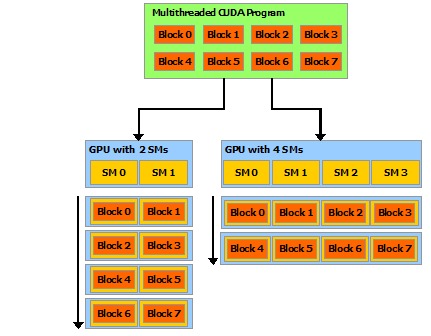
\includegraphics[width=\textwidth]{Documents/Report/Figures/Automatic scalability.png}
\caption{"Automatic scalability of thread blocks. Source: \cite[Figure 3]{nvidia:cudadoc}"}
\label{fig:automatic scalability}
\end{figure}

